% !TEX program = xelatex
\documentclass[11pt,aspectratio=169]{beamer}

\makeatletter
\def\@makefnmark{}
\makeatletter

\setbeamersize{text margin left=5mm,text margin right=5mm} 

\usepackage{amsthm,amsmath,amssymb,braket,fontspec,unicode-math}
\usepackage[absolute,overlay]{textpos}

\usetheme[numbering=none,nofirafonts]{focus}

\setbeamercolor{footnote}{fg=blue}
\setbeamerfont{footnote}{size=\tiny}

\setmainfont{FiraCode Nerd Font}
\setsansfont{Fira Sans}
\setmathfont{Fira Math}
\setmathfont{Latin Modern Math}[range={frak,\bigcap,\bigcup}]
\setbeamerfont{title}{size=\LARGE, shape=\scshape}
\setbeamerfont{author}{size=\large, shape=\scshape}
\setbeamerfont{institute}{size=\normalsize, shape=\scshape}
\setbeamerfont{date}{size=\normalsize, shape=\scshape}
\setbeamerfont{frametitle}{size=\large, shape=\scshape}

\usepackage[backend=bibtex,url=false,doi=false,maxcitenames=1, style=authoryear]{biblatex}
\bibliography{bib}
\AtBeginBibliography{\scriptsize}

\newcommand{\focus}[1]{\textcolor{red}{\bf{#1}}}

\definecolor{red}{HTML}{CC0000}
\definecolor{lred}{HTML}{e24a33}
\definecolor{lblue}{HTML}{348abd}
\setbeamertemplate{bibliography item}[triangle]

\graphicspath{{./figures/}} % Change the path

\AtBeginSection[]{
\begin{frame}
  \vfill
  \centering
  \begin{beamercolorbox}[sep=20pt,rounded=true,center]{frametitle}
    \usebeamerfont{title}\insertsectionhead\par%
  \end{beamercolorbox}
  \vfill
\end{frame}
}
\title{
	{Holographic entanglement in free \\ fermionic quantum matter: hierarchy \& topology}
}
\date{\today}
\author{Abhirup Mukherjee, Siddhartha Patra, Siddhartha Lal}
\institute{Department of Physical Sciences, IISER Kolkata, Mohanpur}
\date{\today}

\begin{document}

\centering

\begin{frame}
\maketitle
\begin{textblock*}{0.4\textwidth}(5.5cm, 6.5cm)
	\centering
	\vspace*{\fill}

	\includegraphics[width=0.35\textwidth]{figures/epqm_logo_mod.jpeg}
	\hspace*{\fill}
	\includegraphics[width=0.35\textwidth]{figures/dps_logo.jpeg}

	\vspace*{\fill}
\end{textblock*}
\end{frame}

\section{Introduction}

\begin{frame}{The system}

\begin{minipage}{0.5\textwidth}
{Massless Dirac fermions on a 2-torus}
\[\mathcal{L} = i\overline\psi\gamma_\mu\partial_\mu \psi\]
{In presence of an Aharonov-Bohm flux}
\[\mathcal{L} = \overline\psi \left(i\gamma_\mu + eA_\mu\right)\partial_\mu \psi\]
\end{minipage}
\begin{minipage}{0.4\textwidth}
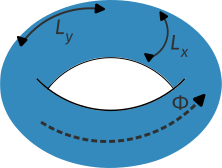
\includegraphics[width=\textwidth]{figures/torus.pdf}
\end{minipage}

\end{frame}

\begin{frame}{Measures of entanglement}
\vspace*{-30pt}
	\begin{minipage}{0.39\textwidth}
	\vspace*{30pt}
	\only<1-4>{
	\(\rho = \ket{\Psi}\bra{\Psi}\longrightarrow\)\focus{density matrix}\\[20pt]
	\only<2->{\(\rho_A = \) partial trace over system A\\
	\(\longrightarrow\) \focus{reduced DM}\\[20pt]}
}
	\end{minipage}
	\hspace*{10pt}
	\begin{minipage}{0.55\textwidth}
		\centering
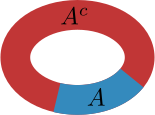
\includegraphics[width=0.49\textwidth]{figures/subsystem-A.pdf}
\includegraphics[width=0.49\textwidth]{figures/subsystem-torus.pdf}
\end{minipage}

\vspace*{\fill}

\only<3>{\(S(A) = -\text{Tr}\left[\rho_A \log \rho_A\right] \longrightarrow\) \focus{entanglement entropy} of A\\[10pt]
\(\longrightarrow\) quantifies information shared between \(A\) and rest}
	\only<4>{\(I(A:B) = S(A) + S(B) - S(A \cup B) \longrightarrow\) \focus{mutual information} between \(A\) and \(B\)\\[10pt]
\(\longrightarrow\) quantifies information shared between \(A\) and \(B\)}
\end{frame}

\begin{frame}{Entanglement of free fermions}
\[\mathcal{L} = i\overline\psi\gamma_\mu\partial_\mu \psi\]
	Diagonal in \(k-\)space \(\mathbf\longrightarrow\) \focus{Vanishing} entanglement in momentum space\\[20pt]
	\only<2>{Off-diagonal in \(r-\)space \(\mathbf\longrightarrow\) \focus{Fluctuations} exist in real space\\
		\(\mathbf\longrightarrow\) leads to entanglement in real space\\[20pt]
	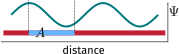
\includegraphics[width=0.6\textwidth]{figures/nonlocal.pdf}}
\end{frame}

\begin{frame}{Entanglement of free fermions}
	Some existing results on fermionic entanglement:\\[10pt]
\begin{itemize}
	\item massless fermion on \(1-\)d line: \(~ ~ ~ \frac{1}{3}\log \left(l/\epsilon\right) \)\\[20pt]
	\item massive fermions on \(1-\)d line: \(~ ~ ~ \frac{1}{3}\log \left(l/\epsilon\right) - \frac{1}{6}\left( ml \log ml \right)^2 \)\\[20pt]
	\item massless fermions in higher dims.: \(~ ~ ~ ~ l^{d-1}\log l\)\\[20pt]
\end{itemize}
\footcite{calabrese2004,Casini_2005,gioev2006,wolf_area_2006,li_scaling_2006,Casini_2009}
\end{frame}

\section{Reduction of \(2-\)D system to \((1+1)-\)D systems}

\begin{frame}{Reduction to \((1+1)-\)D systems}
\footcite{chung_2000,Arias_2015,Chen_2017,Murciano_2020}
	\only<1>{In presence of flux: ~ ~ ~{\Large\(\mathcal{L} = \int dx dy ~ ~ ~\overline\Psi(x) \left(i\gamma_\mu + eA_\mu\right)\partial_\mu \Psi(x)\)}\\[20pt]
	Periodic boundary conditions along \(\vec x\): ~ ~ ~ {\Large \(k_x^n = \frac{2\pi n }{L_x},~ ~ n \in \mathbb{Z} \)}\\[20pt]
	Introduce Fourier modes: ~ ~ ~ {\Large \(\Psi(x) = \sum_{n=-\infty}^\infty e^{i x k_x^n}\Psi(k_x^n)\)}
}
\only<2>{
	Decouples into massive \(1D\) modes: ~ ~ {\large \(\mathcal{L}=\sum_{n} \int dy ~ \overline\Psi(k_x,y) \left(i\gamma_\mu \partial_\mu - M\right) \Psi(k_x, y)\)}\\
	\vspace*{\fill}
Mass of each mode: ~ ~ {\(M(n,\phi) = \frac{2\pi}{L_x}|n + \phi|\)}\\
	\vspace*{\fill}
\includegraphics[width=0.7\textwidth]{figures/dim-reduc.pdf}
}
\only<3>{
	\(2D\) system is described by sum over \(1D\) modes.\\[10pt]
{\LARGE\(\downarrow\)}\\[10pt]
Modes do not couple - no inter-mode entanglement in \(k-\)space\\[10pt]
{\LARGE\(\downarrow\)}\\[10pt]
Total position-space entanglement is sum of each part: ~ {\Large\(S = \sum_n S_n\)}\\[10pt]
	\vspace*{\fill}
\begin{minipage}{0.65\textwidth}
	\[S_n(\phi) = \underbrace{c \log \left(\alpha L_x\right)}_\text{modified area law} - \underbrace{c \log |n + \phi|}_\text{mass correction}\]
\end{minipage}
\begin{minipage}{0.33\textwidth}
\(\alpha\longrightarrow\) non-universal cutoff dependent constant
\end{minipage}
}
\end{frame}

\section{What are we going after?}

\begin{frame}{What are we going after?}
	\begin{itemize}
		\item Distribution of entanglement across subsystems and scales\\[20pt]
		\item Emergent space generated by this entanglement (\focus{holography})\\[20pt]
		\item Curvature and related quantities of this emergent space
	\end{itemize}

\end{frame}

\section{Entanglement hierarchy in mixed momentum and real space}

\begin{frame}{Creating subsystems}
	\[k_x^n = \frac{2\pi }{L_x} n,~ ~ n \in \mathbb{Z};~~~ \text{define \focus{distance}} = \Delta n = 1\]
	\focus{Simplest} choice: the entire set
	\[\text{distance} = 1 \longrightarrow n \in \left\{-N,-(N-1),-(N-2),\ldots,-1,0,1,\ldots,N-2,N-1,N\right\} \]
	\focus{Coarser} choices: increase distance
	\[\text{distance} = 2 \longrightarrow n \in \left\{-N,-(N-2),-(N-4),\ldots,-2,0,2,\ldots,N-4,N-2,N\right\} \]
	\[\text{distance} = 4 \longrightarrow n \in \left\{-N,-(N-4),-(N-8),\ldots,-4,0,4,\ldots,N-8,N-4,N\right\} \]
	\centering
	\vspace*{\fill}
	
\includegraphics[width=0.4\textwidth]{figures/A_mi.pdf}
\end{frame}

\begin{frame}{Sequence of subsystems}
	Define \focus{sequence} of subsystems\\[10pt]
{\large \(~ ~ \mathcal{A}_{z}(j): ~ ~ t_z(j) = 2^{j^z}\)}
\[\text{sequence index:}~ ~ ~ j = 0,1,2,\ldots\]
\[\text{strength of coarse/fine-graining:}~ ~ ~ z = \pm 1,\pm 2,\pm 3,\ldots\]
\begin{minipage}{0.48\textwidth}
\centering
\[ z = 1\]
\includegraphics[width=0.99\textwidth]{./figures/coarse-graining.pdf}
\end{minipage}
\hspace*{\fill}
\begin{minipage}{0.49\textwidth}
\centering
\[ z = -1\]
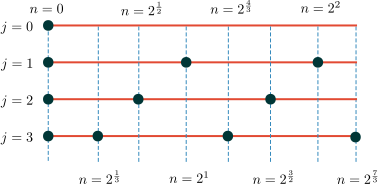
\includegraphics[width=0.99\textwidth]{./figures/fine-graining.pdf}
\end{minipage}
\end{frame}

\begin{frame}{The sequence as a renormalisation group flow}
	Sequence of Hamiltonians {\LARGE \(\longleftrightarrow\)} \focus{renormalisation} group flow\\[10pt]
	RG \(\longrightarrow\) transformation of Hamiltonian via change of scale\\
	\[\text{Superset of all members:}~ ~ ~ \mathcal{A}_z^{(0)} = \bigcup_j \mathcal{A}_z(j)\]
	\[\text{"Super-Hamiltonian":}~ ~ ~\mathcal{H}^{(0)} = \sum_{k_x \in \mathcal{A}_z^{(0)}} \mathcal{H}\left( k_x \right)\]
	\[\text{RG equation:}~ ~ ~\mathcal{H}_z(j) = \underbrace{\mathcal{P}_z(j)}_\text{projector} ~ \mathcal{H}^{(0)} ~ \mathcal{P}_z(j)\]
\end{frame}

\begin{frame}{What, exactly, is getting renormalised?}
	Several ways to look at this\\[10pt]
	\begin{itemize}
		\item renormalisation in \focus{entanglement}: \(\Delta \log S_z(j) \sim \Delta f_z(j) \)\\[10pt]
		\item renormalisation in 1-particle \focus{spectral gap}: \(M(n,\phi) \sim |n + \phi|\)\\[10pt]
		\item renormalisation in real space \focus{quantum fluctuation}\\[10pt]
	\end{itemize}
\end{frame}

\begin{frame}{Fraction of maximum states}
	\centering
	\[f_z(j) = \text{fraction of maximum states} = 1/t_z(j)\]
	\includegraphics[width=0.5\textwidth]{figures/fraction.pdf}
\end{frame}


\begin{frame}{Sequence of subsystems}
\hspace*{\fill}
\begin{minipage}{0.5\textwidth}
Simplest case: \(j=0\)\\[5pt]
\begin{itemize}
	\item no coarse-graining or fine-graining\\[20pt]
	\item \(A_z(0) \longrightarrow ~ ~\)\focus{short cylinder}
\end{itemize}
\end{minipage}
\hspace*{\fill}
\begin{minipage}{0.4\textwidth}
	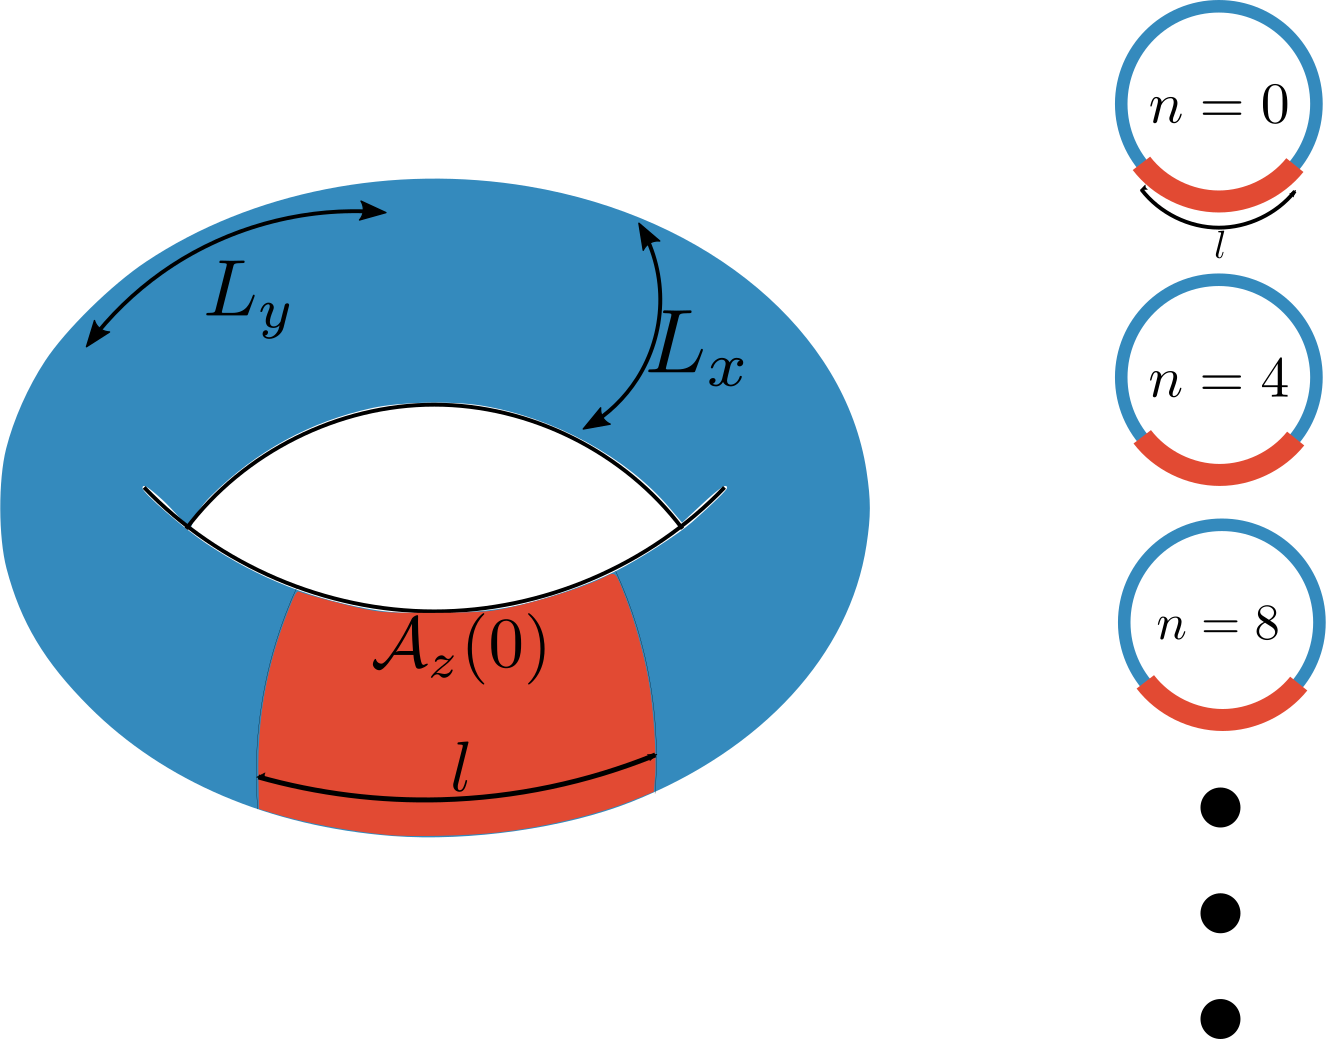
\includegraphics[width=0.8\textwidth]{figures/A_m1.pdf}
\end{minipage}

\vspace*{\fill}
\centering
In general:

\begin{minipage}{0.33\textwidth}
	\[\Delta n \sim \Delta k_x \sim 1/L_x ~ ~ ~\longrightarrow \]
\end{minipage}
\begin{minipage}{0.33\textwidth}
	\[ z > 0: \text{decreasing system size}\]
	\[ z < 0: \text{increasing system size}\]
\end{minipage}
\end{frame}

\begin{frame}{Subsystem entanglement entropy}
\footcite{Calabrese_2004,Casini_2005,Arias_2015,Chen_2017,Murciano_2020}
Modes are decoupled \(\longrightarrow\) entanglement is additive
\vspace*{\fill}
\[S_{\mathcal{A}_z(j)} = \sum_{n \in \mathcal{A}_z(j)} S_n = f_z(j) c \alpha L_x - c \log \big|2\sin\left(\pi f_z(j)\phi\right)\big|\]
\[i < j, ~ ~ S_{i\cup j} =
	\begin{cases}
	S_{i}, ~ ~ z > 0\\
	S_{j}, ~ ~ z < 0
	\end{cases}
\]
\end{frame}
	
\begin{frame}{Entanglement hierarchy}
\begin{minipage}{0.5\textwidth}
\[i < j, ~ ~ S_{i\cup j} =
	\begin{cases}
	S_{i}, ~ ~ z > 0\\
	S_{j}, ~ ~ z < 0
	\end{cases}
\]
\end{minipage}
\begin{minipage}{0.45\textwidth}
\includegraphics[height=0.3\textheight]{figures/Matroshka.png}
\includegraphics[height=0.3\textheight]{figures/nested.png}
\end{minipage}

\vspace*{\fill}

\begin{itemize}
	\item 
presents a \focus{hierarchy} of entanglement \(\longrightarrow\) EE distributed across RG steps:\\[10pt]
RG transformation \(\longrightarrow\) reveals entanglement

\vspace*{\fill}
\item distribution of entanglement also present in \focus{multipartite} entanglement:\\[10pt]
	mutual information and higher order measures, within one RG step or spread across the flow
\end{itemize}

\end{frame}

\section{Holographic nature of the RG flow}
\begin{frame}{Holographic principle}
Conformal FT in \(d-\)dimensions \(\longleftrightarrow\) Anti-de-Sitter space-time in \(d+1\)-dimensions\\[10pt]
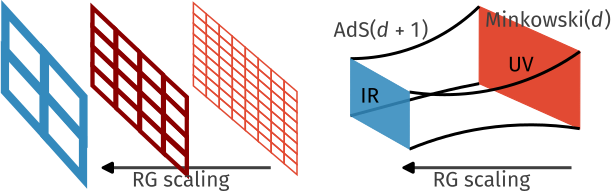
\includegraphics[width=0.9\textwidth]{figures/holography.pdf}\\[10pt]
extra dimension in bulk corresponds to \focus{RG flow}
\footnote{J. McGreevy (McGreevy,2010)}
\end{frame}
\begin{frame}{Mutual information = distance}
\footcite{van2010building,lee2016,anirban_mott_2022}
	\focus{Mutual information}: ~ \(I^2(A:B) \equiv S(A) + S(B) - S(A \cup B)\) ~ ~ ~ (non-negative)\\[10pt]
	information gained about \(B\) upon measuring \(A\)\\[10pt]
	define distance along the RG: ~ ~ \(d_z(j) \equiv \log I^2_\text{max} - \log I_z^2(0:j) = \log t_z(j)\)

	\vspace*{\fill}

	\begin{minipage}{0.4\textwidth}
	\includegraphics[width=\textwidth]{figures/distance1.pdf}
	\end{minipage}
	\hspace*{\fill}
	\begin{minipage}{0.55\textwidth}
		\centering
		For \(z > 0\):\\[5pt]
		\begin{itemize}
			\item mut. info. is maximum for small \(j\)\\[10pt]
			\item decreases for large \(j\)\\[10pt]
			\item corresponds to \focus{increasing distance}
		\end{itemize}
	\end{minipage}
\end{frame}

\begin{frame}{RG evolution = emergent distance}
	\footcite{lee2010,lee2014,qi2013,lee2016,anirbanurg1,anirbanurg2,ryu2006,ryu2006aspects,nozaki2012}
\only<1>{
	Define \(2-\)dimensional \(x-y\) structure\\[20pt]
	\begin{minipage}{0.55\textwidth}
	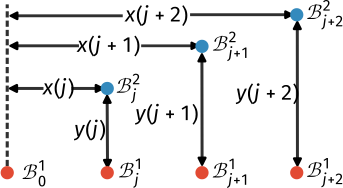
\includegraphics[width=\textwidth]{figures/curvature-scheme.pdf}
	\end{minipage}
	\hspace{\fill}
	\begin{minipage}{0.4\textwidth}
		\centering
	{\color{lred}\circle*{10}}: RG steps\\[10pt]
	{\color{lblue}\circle*{10}}: subsystems within an RG step\\[30pt]

	\(x_z(j) = d_z(j) = \log t_z(j)\)\\

	\[y_z(j) = \log I^2_\text{max} - \log I_z^2(\mathcal{B}_j^1:\mathcal{B}_j^2)\]
\[= \log t_z(j \pm 1)\]
	\end{minipage}
}
\only<2>{
	Define coupling that measures spectral gap:~ ~ \(g_z(j) = \log \frac{M_{n+1}(\phi) - M_n(\phi)}{2\pi/L_x} = \log t_z(j)\)\\[10pt]
	RG beta function for its evolution: ~ ~ \(\beta_z(j) = \Delta \log g_z(j) = z \log\left( 1 + j^{-1} \right) \)

	\includegraphics[width=0.45\textwidth]{figures/coupling.pdf}
	\hspace*{30pt}
	\includegraphics[width=0.45\textwidth]{figures/mass-beta.pdf}
}
\only<3>{
	RG beta function can be related to the \(x,y-\)distances
	\[x_z = \left( e^\frac{\beta_z}{z} - 1 \right)^{-z} \log 2\]
	\[y_z = \begin{cases}
		x_z e^\beta,~~ &z > 0\\
		x_z \left(2 - e^\frac{\beta}{z}\right)^z,~~ &z < 0\\
	\end{cases}\]
	\\[10pt]
	explicit relation between the RG flow and the emergent \focus{geometry}
}
\end{frame}

\begin{frame}{Curvature of the emergent space}
	Define first and second derivatives in emergent space
	\[v_z(j) \equiv \frac{\Delta y_z(j)}{\Delta x_z(j)} =\begin{cases}
		\frac{\left(j+2\right)^z - \left(j+1\right)^z}{\left(j+1\right)^z - j^z},~ ~ z > 0\\
		\frac{\left(j\right)^z - \left(j-1\right)^z}{\left(j+1\right)^z - j^z},~ ~ z < 0\\
	\end{cases}
\]
\[
	v^\prime_z(j) \equiv \frac{v_z(j+1) - v_z(j)}{x_z(j+1) - x_z(j)}
\]
Define curvature using them: {\Large\(\kappa_{z}(j) = \frac{v^\prime_z(j)}{\left[1 + v_z(j)^2\right]^\frac{3}{2}}\)}\\[10pt]
\(\longrightarrow\) can be expressed in terms of \(\beta_z(j)\)
\end{frame}

\begin{frame}{Curvature of the emergent space}
\begin{minipage}{0.45\textwidth}
	\includegraphics[width=\textwidth]{figures/curvature-pos.pdf}
\end{minipage}
\begin{minipage}{0.5\textwidth}
	\begin{itemize}
		\item positive curvature for \(z < 0\)\\[10pt]
		\item zero curvature for \(z = 1\)\\[10pt]
		\item negative curvature for \(z  > 1\)\\[10pt]
		\item \focus{asymptotically flat} for large \(j\), at all \(z\)
	\end{itemize}
\end{minipage}

\vspace*{\fill}
{\it Is there a name for such spaces?}
\end{frame}

\begin{frame}{The sign of the curvature is topological}
\only<1>{
	\[\gamma_z(j) \equiv 1 - v_z(j+1)/v_z(j), ~ ~ ~\alpha_z(j) = y_z(j+1) - y_z(j)\]

\vspace*{\fill}

	\[\kappa_{z}(j) = -\frac{\alpha_z(j)~\gamma_z(j)}{\left(\Delta x_z(j)\right)^2\left[1 + v_z(j)^2\right]^\frac{3}{2}} \implies \text{sign}\left[\kappa_z(j)\right] = -\text{sign}\left[\alpha_z(j)\right]\text{sign}\left[\gamma_z(j)\right]\]

\vspace*{\fill}
\[
	\text{sign}\left[\kappa_z\right] = \begin{cases}
		-1 ,~ ~ z \geq 1\\
		1 ,~ ~ ~ ~ z \leq -1\\
	\end{cases} = ~ ~ \begin{cases}
		-\text{sign}\left[\gamma_z(j)\right] ,~ ~ z \geq 1\\
		-\text{sign}\left[\alpha_z(j)\right] ,~ ~ z \leq -1\\
	\end{cases}
\]

}
\only<2>{
\begin{minipage}{0.49\textwidth}
\includegraphics[width=0.9\textwidth]{figures/gamma.pdf}
\end{minipage}
\begin{minipage}{0.49\textwidth}
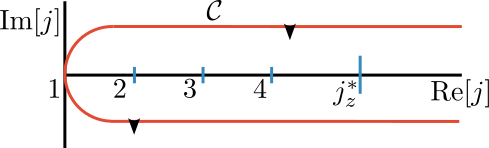
\includegraphics[width=0.9\textwidth]{figures/curvature-contour.pdf}
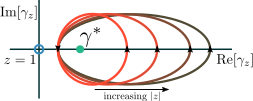
\includegraphics[width=0.9\textwidth]{figures/curvature-winding.pdf}
\end{minipage}\\[10pt]

\begin{itemize}
	\item \(\ln \left(\gamma - \gamma^*\right)\) has branch point at \(\gamma^*\), can be avoided for \(z=1\), \focus{contour is trivial}\\[10pt]
	\item cannot be avoided for \(z \neq 1\) \(\longrightarrow\) presence of \focus{singularity} \(\longrightarrow\) encoded through \focus{winding number}
\end{itemize}


}
\only<3>{
\begin{minipage}{0.5\textwidth}
\includegraphics[width=0.8\textwidth]{figures/alpha.pdf}
\end{minipage}
\begin{minipage}{0.49\textwidth}
	very similar thing holds for \(\alpha_z\)\\[5pt]
	\begin{itemize}
		\item singularity exists only for \(z < 0\)\\[10pt]
		\item otherwise contour can be trivialised
	\end{itemize}
\end{minipage}

\vspace*{\fill}

\includegraphics[width=0.6\textwidth]{figures/alpha-winding.pdf}
}
\only<4>{
	Curvature can be written as the product of \focus{winding numbers}:

	\[\text{sign}\left[\kappa_z\right] = \mathcal{W}_z\left( \gamma^* \right) \times \left[2\mathcal{W}^\prime_z\left( \alpha^* \right) - 1\right] \]\\[20pt]

	\begin{itemize}
		\item winding numbers count singularities\\[10pt]
		\item robust against deformations
	\end{itemize}
	
}
\only<5>{
	{\it What does this change in topology really mean?}
	\vspace*{\fill}
	\begin{itemize}
		\item \(z\) is the \focus{anomalous dimension} of the spectral gap \(g_z\) in the effective field theory\\[20pt]
		\item sign of \(z\) reflects the RG relevance/irrelevance of \(g_z\) in the microscopic fermionic theory\\[20pt]
		\item change in \(z\) can be interpreted as a change in the underlying \focus{interacting theory}\\[20pt]
		\item change in sign of \(z\) is hence a \focus{phase transition} in the microscopic theory that changes the topology of the Fermi surface
	\end{itemize}
}
\end{frame}

\begin{frame}{Evolution of expansion parameter}
\footcite{kar_2001,kar2007raychaudhuri,balasubramanian1999}
\only<1>{
\begin{minipage}{0.6\textwidth}
\begin{itemize}
	\item Define an expansion parameter\\[20pt]
	\item can be related to RG flow through \(\beta_z\)\\[20pt]
	\item related to change in area of flows of \(g_z\)
\end{itemize}
\end{minipage}
\begin{minipage}{0.35\textwidth}
	\[\theta_z(j) = \frac{1}{\sqrt{1 + v_z^{-2}}}\]\\
\[\theta_z \sim \frac{1}{\sqrt{\Delta x^2 + \Delta y^2}}\Delta g_z(j+1)\]
\end{minipage}
}
\only<2>{
\begin{minipage}{0.5\textwidth}
	\begin{itemize}
	\item Expansion parameter satisfies "Raychaudhuri-like" equation
	\[\frac{\:\mathrm{d}\theta_z}{\:\mathrm{d}x_z} = \kappa\]\\[10pt]
\item No attractive \(\theta^2\) term: fixed points reached only at \(j \to \infty\)\\[20pt]
	\end{itemize}
\end{minipage}
\begin{minipage}{0.45\textwidth}
\includegraphics[width=0.99\textwidth]{figures/theta.pdf}
\end{minipage}
}
\end{frame}

\section{Conclusions}
\begin{frame}{Conclusions}
	\begin{itemize}[<+-|alert@+>]
		\item hierarchy of entanglement, across scales as well as number of parties\\[20pt]
			\only<1>{
			\[S_{A \cup B} = S_{\text{larger}}\]}
		\item RG beta function gives rise to emergent distances\\[20pt]
			\only<2>{
			\[x_z(\beta), y_z(\beta)\]}
		\item anomalous dimension \(z\) determines sign of curvature\\[20pt]
			\only<3>{
			\[\kappa \begin{cases}
				> 0 \text{ if }z < 0\\
				= 0 \text{ if }z = 1 \\
				< 0 \text{ if }z > 1 \\
			\end{cases}\]}
		\item sign of curvature is topological\\[20pt]
			\only<4>{
			\[\text{sign}\left[\kappa_z\right] = \mathcal{W}_z\left( \gamma^* \right) \times \left[2\mathcal{W}^\prime_z\left( \alpha^* \right) - 1\right] \]}
		\item \(\theta\) satisfies "Raychaudhuri-like" equation
			\only<5>{
			\[\frac{\:\mathrm{d}\theta_z}{\:\mathrm{d}x_z} = \kappa\]}
	\end{itemize}
\end{frame}

\begin{frame}[allowframebreaks]{References}
\printbibliography
\end{frame}

\begin{frame}{Other Stuff}

\begin{minipage}{0.5\textwidth}
\begin{itemize}
\item Transformation to a different space
	\[ \tilde\theta = \frac{1}{1 - \sqrt 2 \theta}, ~ ~ ~ ~\frac{\:\mathrm{d}\tilde\theta}{\:\mathrm{d}x_z} = \sqrt 2 \tilde\theta^2 \kappa \]\\[5pt]
\item Does generate \(\theta^2\) term\\[10pt]
\item Effective curvature is zero
\end{itemize}
\end{minipage}
\begin{minipage}{0.49\textwidth}
\includegraphics[width=0.99\textwidth]{figures/thetap.pdf}
\end{minipage}
\end{frame}

\end{document}
